\documentclass[a4paper, oneside, nobib, notoc, justified]{tufte-book}

% Load packages
\usepackage{graphicx}
\usepackage{tikz}
\pgfrealjobname{fig}
\usepackage{amsmath,amssymb}
\usepackage{relsize}
\usepackage[smaller]{acronym}

% Commands
\newcommand{\ft}[0]{\footnotesize}
\newcommand{\scs}[0]{\scriptsize}
\newcommand{\sm}[0]{\small}

% Acronyms
\newacro{HRTF}[HRTF]{head-related transfer function}
\newacro{SSR}[SSR]{SoundScape Renderer}
\acronymused{HRTF}
\acronymused{SSR}

\begin{document}
    \beginpgfgraphicnamed{fig4_01}
    \small
    \begin{tikzpicture}
        \draw (0,0)       node {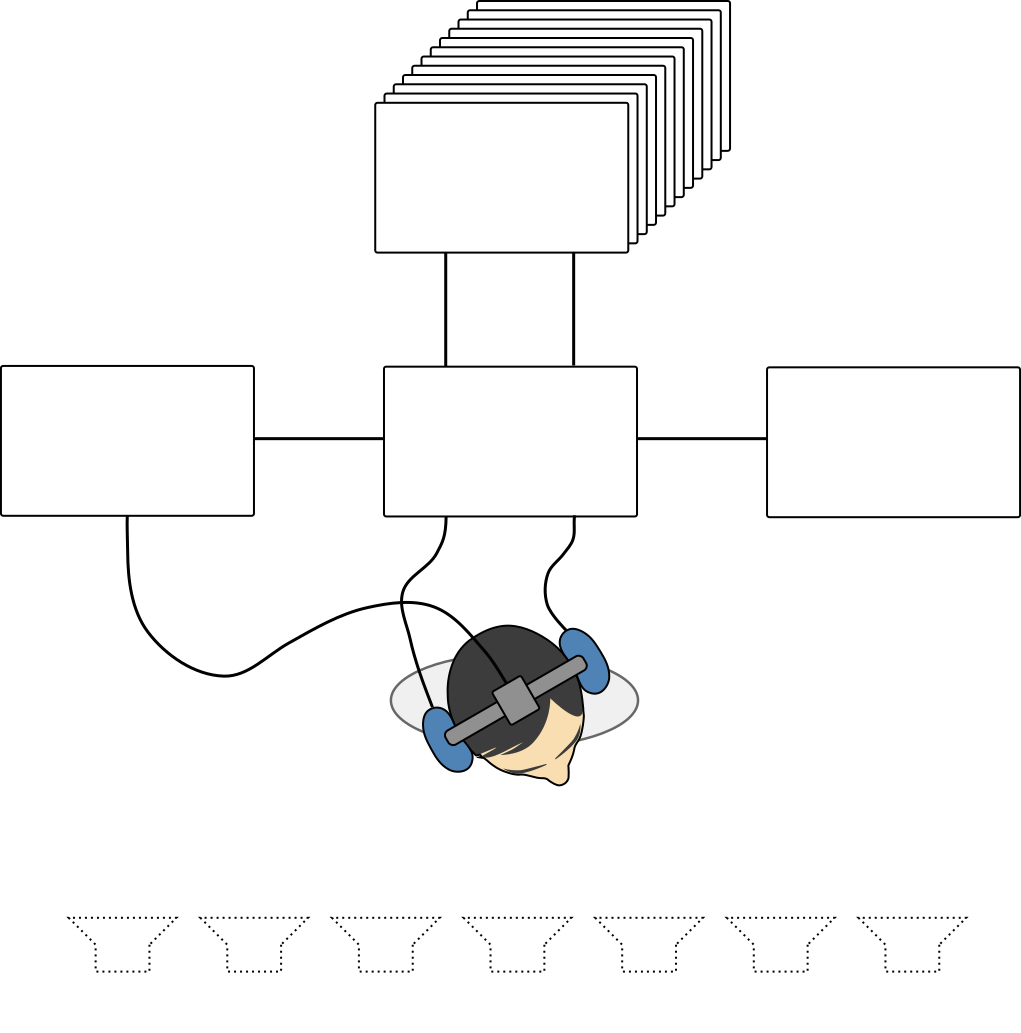
\includegraphics[width=.8\columnwidth]{src/dynamic_binaural_synthesis}};
        \draw (-0.06,2.9) node {\acs{HRTF}};
        \draw (-0.06,2.4) node {\scs\shortstack{for \\head orientation $\phi$}};
        \draw (0,0.7)     node {\acs{SSR}};
        \draw (0,0.1)     node {\scs\shortstack{convolution and \\ \acs{HRTF} switching}};
        \draw (-3.2,0.7)  node {\ft head tracker};
        \draw (-3.2,0.1)  node {\scs\shortstack{ head orientation $\phi$}};
        \draw (3.2,0.4)   node {\ft\shortstack{dry \\ audio material}};
        \draw (0,-4.5)    node {\ft simulated loudspeakers};
    \end{tikzpicture}
    \endpgfgraphicnamed
\end{document}
